\subsection{Analysis Tools}
\subsubsection{Group Participation Impact Tool}
The Group Participation Impact Tool (GAIT) is used for monitoring the relative workload of all members of a team. 
This will assist in evenly distributing the workload, possibly increasing the overall productivity of the team. 
Additionally the tool exposes any team members that are less productive than what is expected. 
Every task has to be manually weighted to reflect the difficulty and workload of the task. 
If the difficulty or workload of a task is under- or over-estimated the reflection of the workload of the members given by the tool will not be correct.
This tool has been used only sparingly throughout the course of the project. 
Very often it has been hard to identify individual tasks and harder still to determine the importance/weight of each task. 
These difficulties meant that any benefits of distributing tasks using the tool did not compensate for the extra time associated with using the tool. 
% [Is the following reasonable?] 
% I think it is - Nikolaj
By not using any structured method of distributing tasks, other than identifying tasks (where possible) and people volunteering for any task that they find interesting, we may have skewed the relative workload of the members. 
Certainly it has meant that some people have worked almost exclusively on one subject.
\begin{landscape}
	\begin{figure}[h!]
		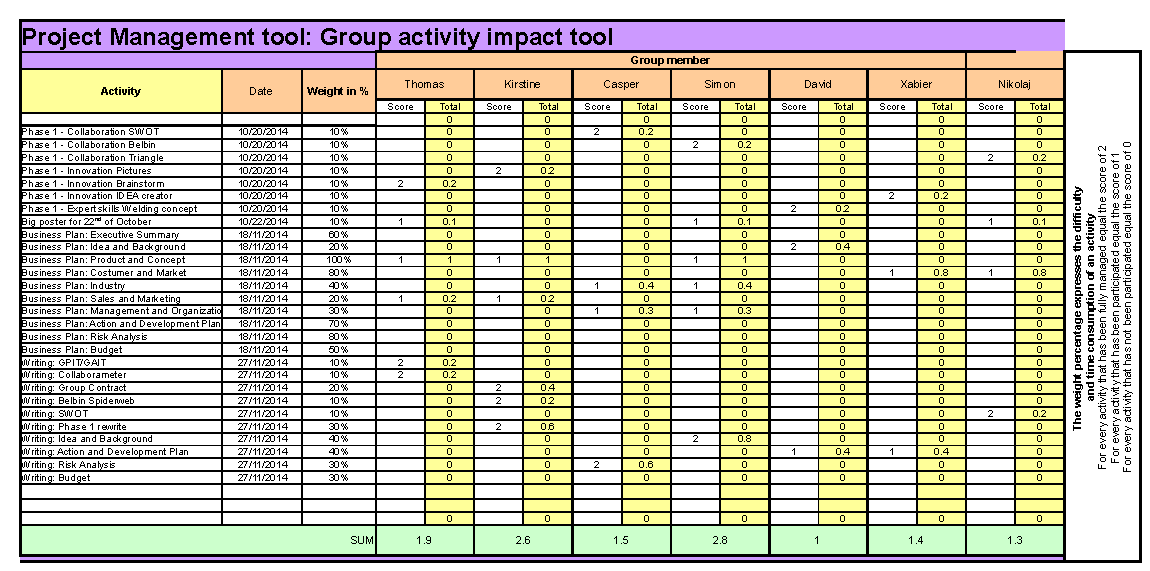
\includegraphics[scale=1.25]{./graphics/GAIT}
		\caption{The GAIT tool with all the entries made by the group}
		\label{fig:GAIT}
	\end{figure}
\end{landscape}
\subsubsection{Group Activity Impact Tool}
The Group Activity Impact Tool (GPIT) is simply a tool for monitoring the meeting participation of each individual member. 
It provides a graphical representation of the participation. Using this tool will provide the team with concrete evidence of the participation of each member. 
This could prove useful, should a situation where a team members contribution is in question arise. 
It looks at the participation in relation to how often people show up and compares that to the the weight of the jobs each member performs.
Based on the weight of the work each member do and how often they attend to meetings each member will be given a score. 
This participation score shows how much each member works on the project and actions can be taken if someone doesn't collaborate with the group at all. 
The scores for each member can be seen in figure \ref{fig:GPITGraph}.

% The participation table can be seen in \ref{fig:GPIT}.

% \begin{figure}[h!]
% 	\makebox[\textwidth][c]{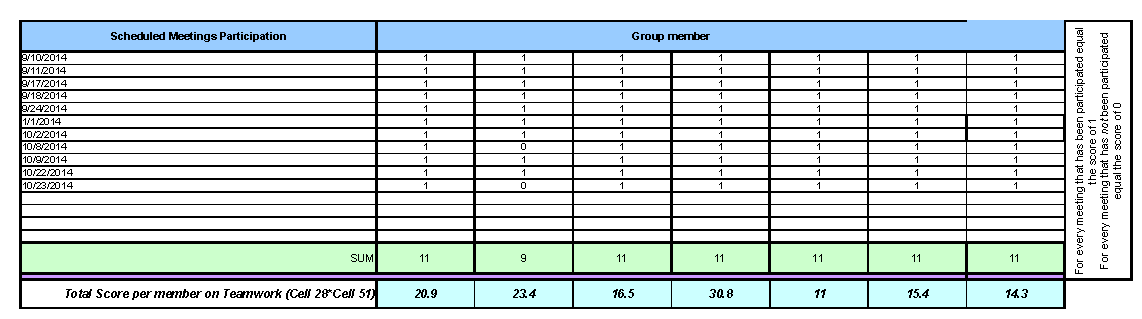
\includegraphics[scale=0.85]{./graphics/GPIT}}
% 	\caption{The GPIT tool }
% 	\label{fig:GPIT}
% \end{figure}

\begin{figure}[h!]
	\makebox[\textwidth][c]{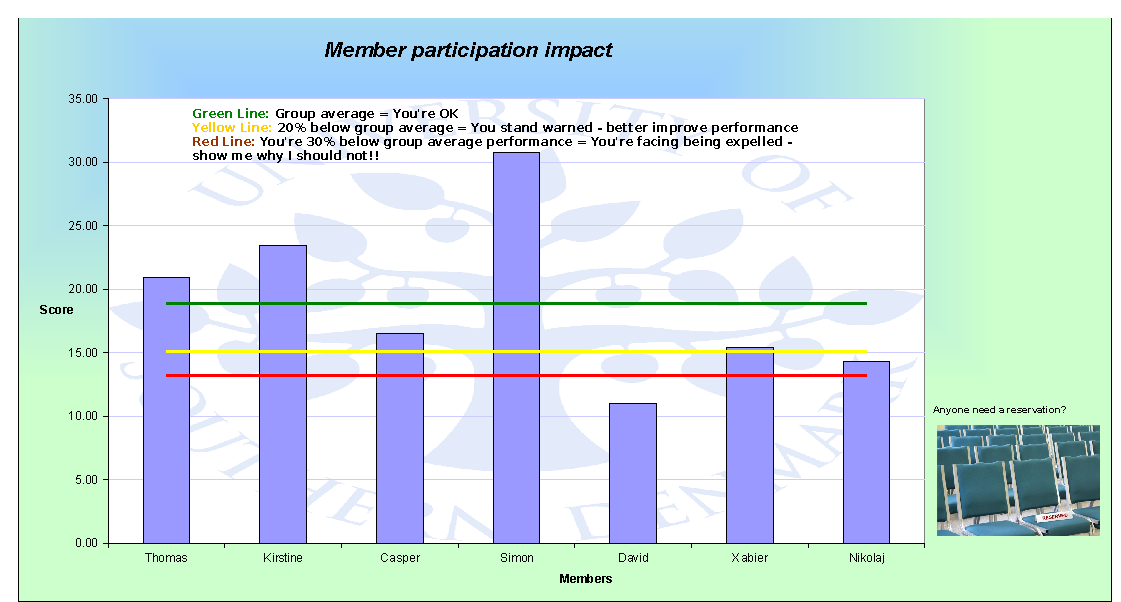
\includegraphics[scale=0.86]{./graphics/GPITGraph}}
	\caption{The impact from each member}
	\label{fig:GPITGraph}
\end{figure}